%%%%%%%%%%%%%%
% Evaluation %
%%%%%%%%%%%%%%

\chapter{Evaluation}
\label{chapter:evaluation}

\section{Erfüllung der Kriterien}

% Kriterien aus Abschnitt \ref{sec:criteria}

\begin{enumerate}[label={K.\arabic*}]

\item
\label{eval:gui}
\textbf{GUI}

\item
\label{eval:interactivity}
\textbf{Interaktivität}

\item
\label{eval:immediate-feedback}
\textbf{Unmittelbares Feedback}

\item
\label{eval:editing-support}
\textbf{Förderung des Prozesses der Diagramm-Erstellung}

\item
\label{eval:mental-map}
\textbf{Erhaltung des mentalen Modells}

\item
\label{eval:focus-on-the-content}
\textbf{Förderung der Konzentration auf den Inhalt}

\item
\label{eval:aesthetics-criteria}
\textbf{Berücksichtigung der ästhetischen Prinzipien}

% ästhetische Prinzipien in K.7

\item
\label{eval:syntax-and-semantics}
\textbf{Berücksichtigung der Syntax und Semantik}

\item
\label{eval:user-friendly}
\textbf{Benutzerfreundlichkeit}

\end{enumerate}

% kleine Diagramme sind schnell zu zeichnen, manuelle Bearbeitung skaliert nicht mit der Größe des Diagramms \cite{Eichelberger05Aesthetics}
% -> Problem, wenn viele Klassen im Diagramm

\section{Nutzerstudie}

Um das umgesetzte Konzept zu validieren, wurde im Rahmen der Bachelor-Arbeit eine Nutzerstudie durchgeführt, die den Gegenstand für die folgenden Abschnitte bildet. Zunächst werden in Abschnitt \ref{subsec:user-study-setup} der Aufbau und die Durchführung im Detail erläutert. Anschließend folgt in Abschnitt \ref{subsec:user-study-evaluation} eine Auswertung der Ergebnisse.

\subsection{Aufbau und Durchführung}
\label{subsec:user-study-setup}

Die Nutzerstudie wurde in individuelle Sitzungen aufgeteilt. Jede Sitzung hat mit einer kurzen Beschreibung des Themas der Bachelor-Arbeit angefangen. Danach wurde der Ablauf der Sitzung vorgestellt und der Teilnehmer wurde um das Ausfüllen des ersten Teils des vorgefertigten Fragebogens (siehe Abschnitt \ref{sec:user-study-material-questionnaire}) gebeten, in dem allgemeine Informationen und Vorkenntnisse abgefragt wurden. Nach Bedarf wurde anschließend eine kurze Einführung über Klassendiagramme gegeben, um die Notation und die wichtigsten Begriffe wie Klasse, Vererbung, Oberklasse und Unterklasse zu erklären.

Die eigentlichen Tests des entwickelten Prototyps (siehe Kapitel \ref{chapter:prototype}) wurden an einem \textit{MacBook Pro} durchgeführt. Als Eingabegerät stand den Teilnehmern das in dem Notebook eingebaute Trackpad, eine \textit{Apple Magic Mouse}\footnote{\url{https://www.apple.com/magicmouse}} und eine klassische optische Maus zur Verfügung. Um potenzielle Probleme mit der Eingabe zu vermeiden, konnten die Teilnehmer frei das passende Eingabegerät wählen.

Als Nächstes wurde eine kurze Einführung zu dem Prototyp gegeben. Die unterstützten Aktionen wie das Erstellen bzw. Umbenennen einer Klasse, Erstellen einer Vererbungsrelation und Löschen des Diagramms wurden beschrieben und im Prototyp demonstriert. Insbesondere wurden die zwei Möglichkeiten zum Erstellen der Vererbungsrelation gezeigt, nämlich durch das Anklicken des Icons in der Sidebar und durch das Drücken der der Taste \texttt{CTRL} (siehe Abschnitt \ref{subsec:supported-actions}). Nach dieser Einführung durfte der Teilnehmer den Prototyp für ca. zwei Minuten ausprobieren.

Der eigentliche Test bestand darin, vier verschiedene Aufgaben zur Modellierung von Klassendiagrammen mit Vererbungshierarchien zu erfüllen. Alle Aufgaben haben das baumbasierte Layout benötigt, so dass die Lay\-out-Engine nicht geändert werden musste. Dem Teilnehmer wurden nacheinander Blätter mit den Aufgabenstellungen vorgelegt, die durch ihn gelöst wurden. Zum einen handelte sich um visuelle Aufgaben, in den der Teilnehmer ein bestehendes Diagramm rekonstruieren sollte. Zum anderen hatten die Aufgaben die Form einer textuellen Beschreibung. Alle Aufgabenblätter sind im Anhang unter Abschnitt \ref{sec:user-study-material-task-description} abgebildet.

Die Teilnehmer wurden gebeten, während der Erfüllung der Aufgaben ihr Vorgehen laut zu beschreiben. Dabei wurden die wichtigsten Beobachtungen notiert. Weiterhin wurde der Bildschirm aufgenommen, um eventuelle weitere Analysen zu ermöglichen. Die Videodateien sind auf der beigelegten DVD zu finden (für das Dateienverzeichnis siehe Abschnitt \ref{sec:files-user-study}).

Im Anschluss wurde das Konzept durch den Teilnehmer bewertet, indem der verbleibende Teil des Fragebogens (siehe Abschnitt \ref{sec:user-study-material-questionnaire}) ausgefüllt wurde. Obwohl die Teilnehmer in den letzten Fragen des Fragebogens eine Möglichkeit hatten, ein allgemeines Feedback zu geben, wurde in einzelnen Fällen eine Diskussion bevorzugt.

\subsection{Auswertung}
\label{subsec:user-study-evaluation}

An der Nutzerstudie haben insgesamt 7 Testpersonen teilgenommen und beide Geschlechter wurden ungefähr gleichmäßig vertreten (4 männliche und 3 weibliche Teilnehmer). Großteils handelte sich um Studenten und wissenschaftliche Arbeiter zwischen 21 und 34 Jahren. Des Weiteren waren 6 von 7 Teilnehmern im Bereich der Informatik tätig und waren daher mit der Notation von Klassendiagrammen vertraut.

\begin{figure}
\centering
\begin{minipage}{.15\textwidth}
    \centering
    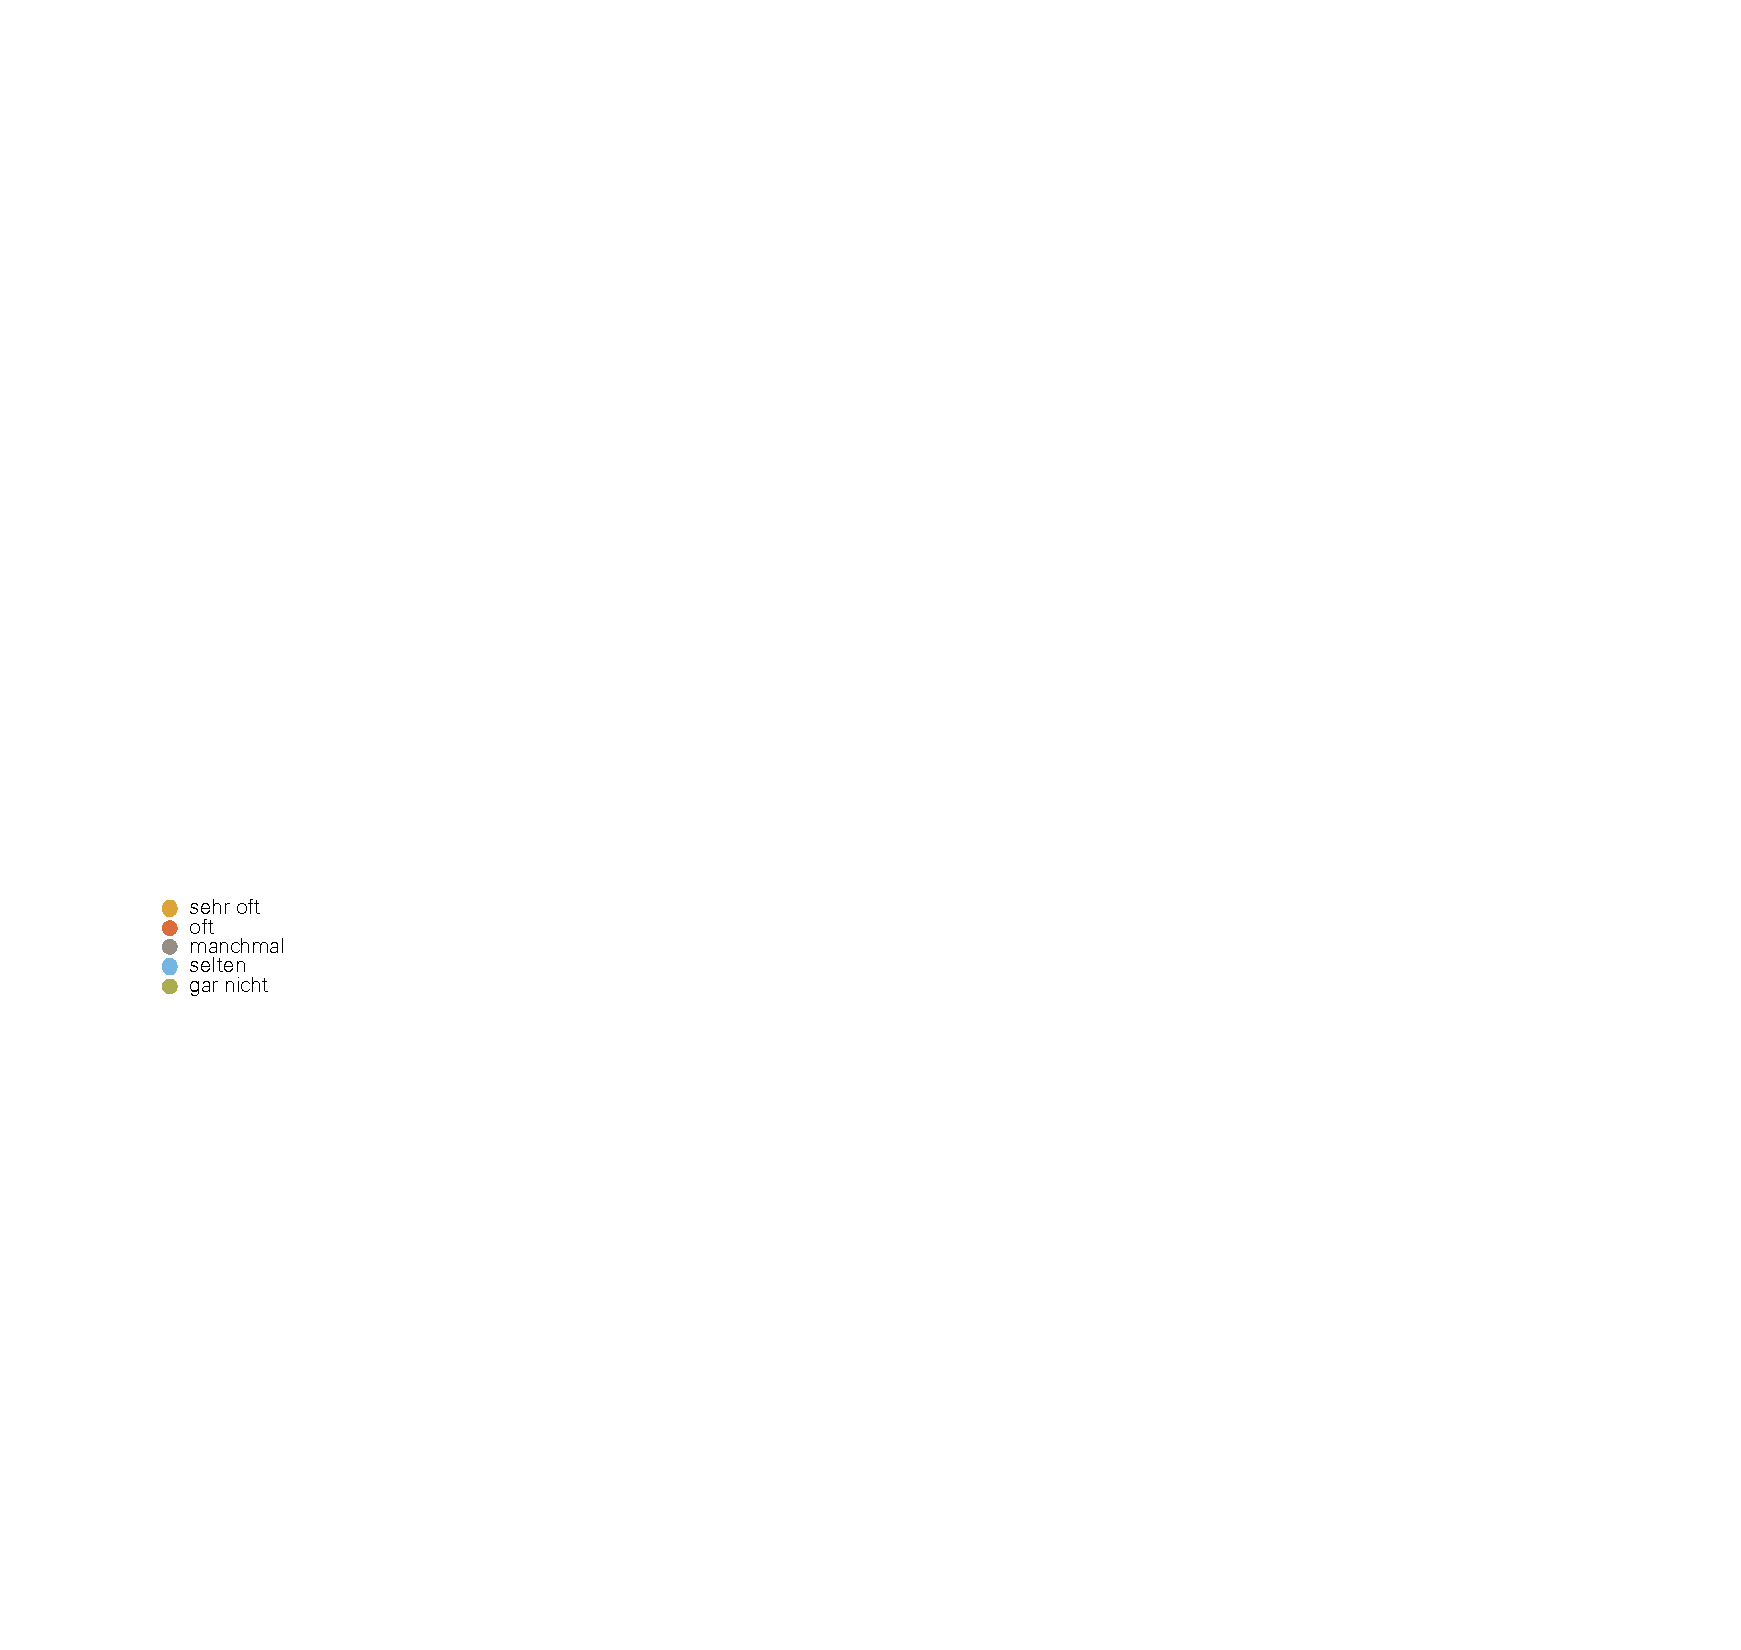
\includegraphics[width=\linewidth]{resources/used-tools-legend}
\end{minipage}
\begin{minipage}{.65\textwidth}
    \newcommand{\subfigurewidth}{0.3\linewidth}
    \newcommand{\graphicsscale}{0.8}
    \centering
    \begin{subfigure}{\subfigurewidth}
        \centering
        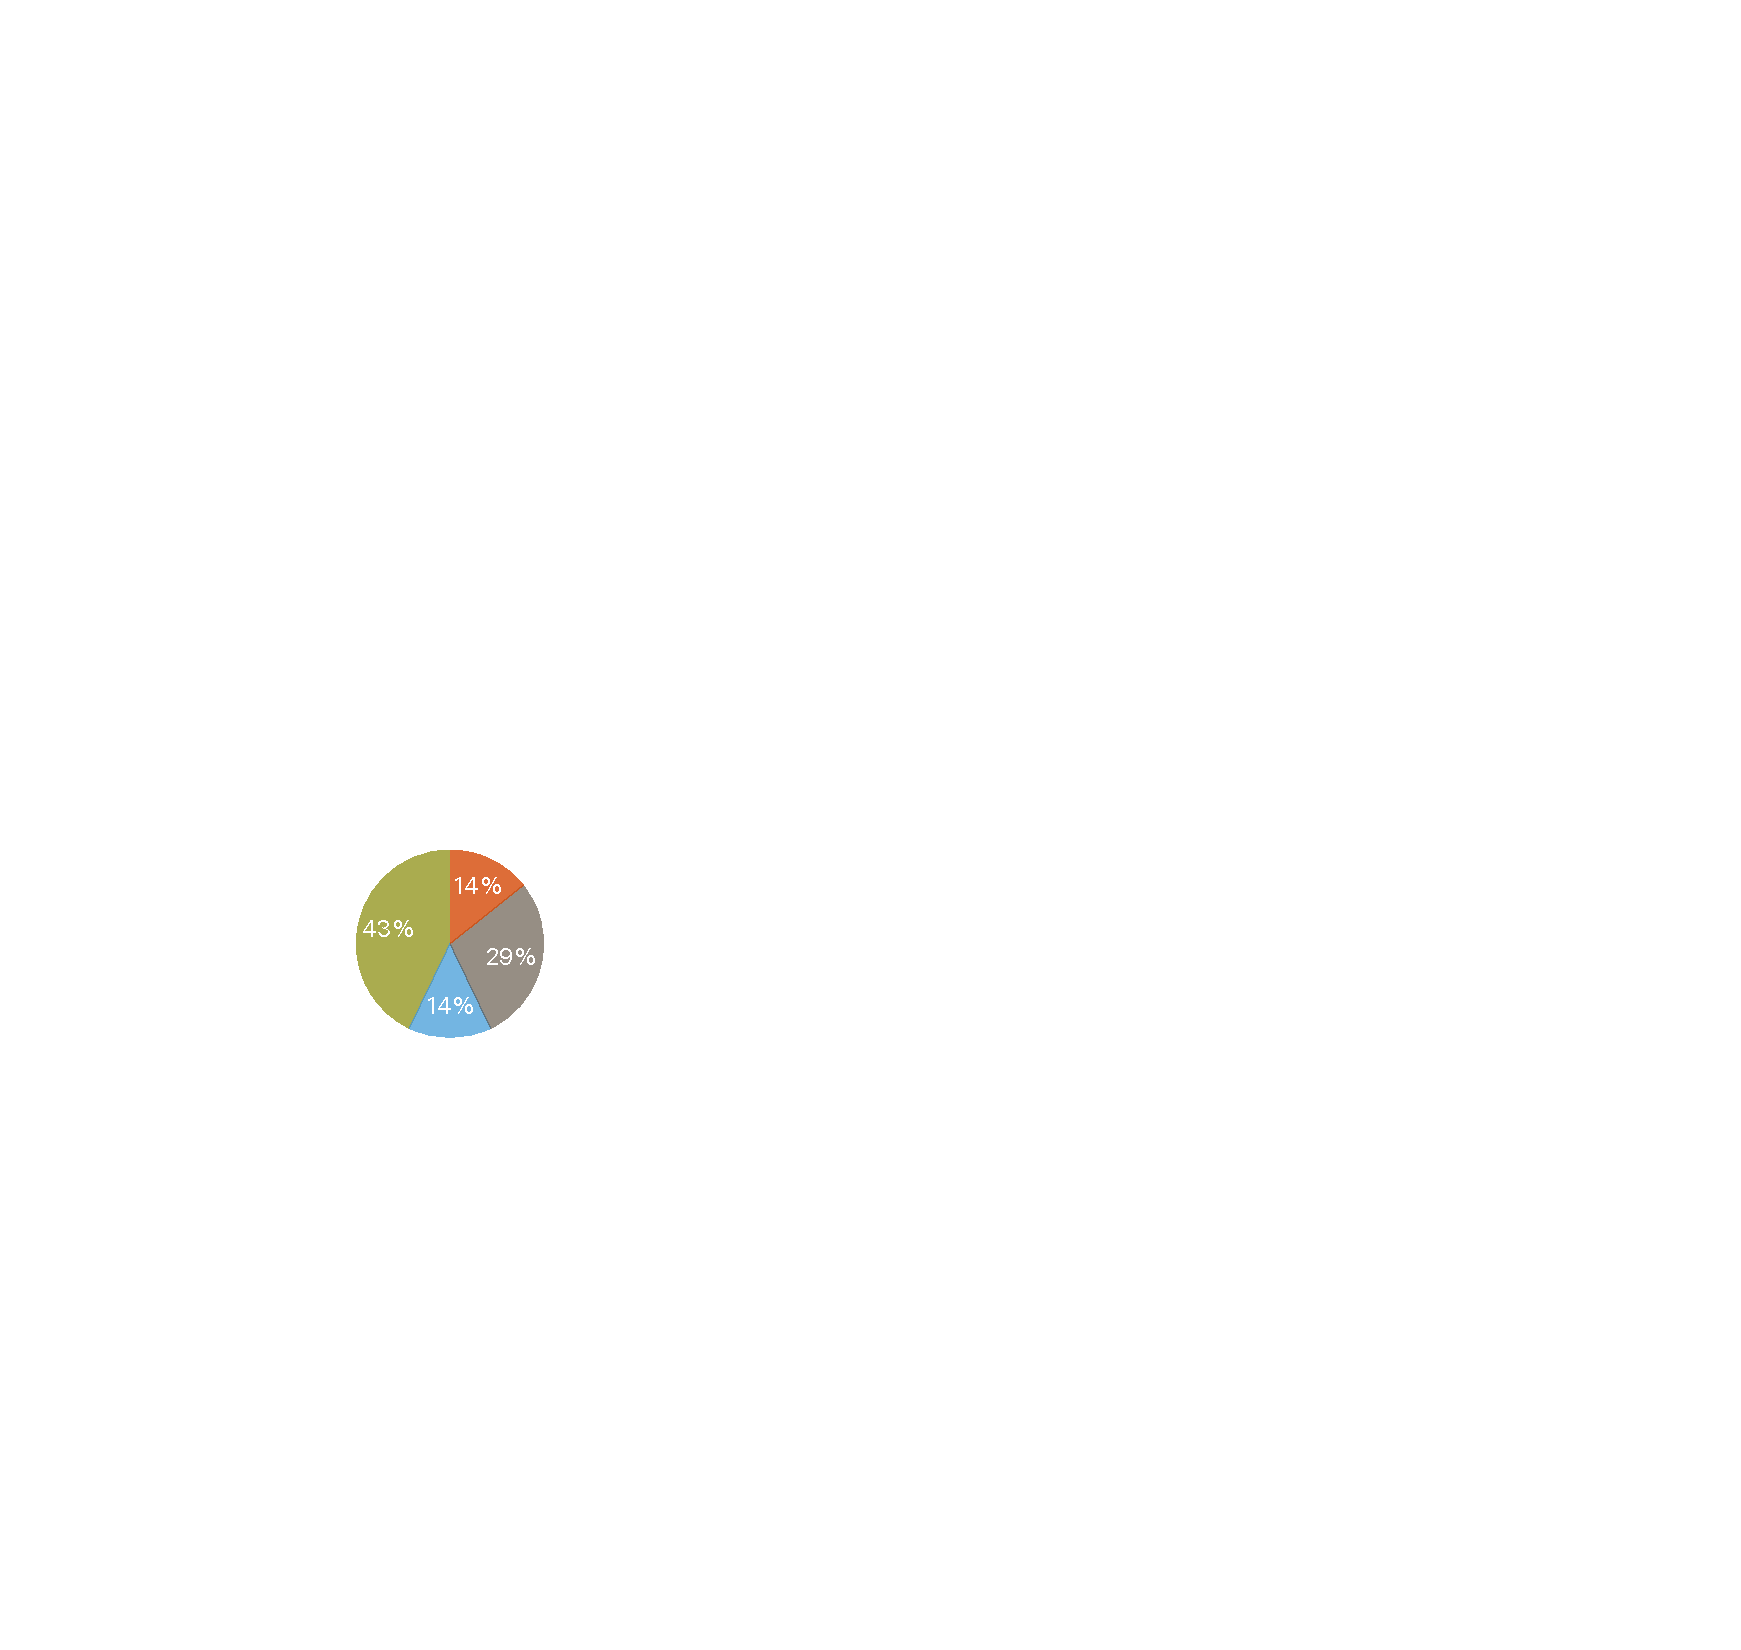
\includegraphics[scale=\graphicsscale]{resources/used-tools-charts-a}
        \caption{Diagramm-Programme}
        \label{fig:used-tools-charts-a}
    \end{subfigure}
    \begin{subfigure}{\subfigurewidth}
        \centering
        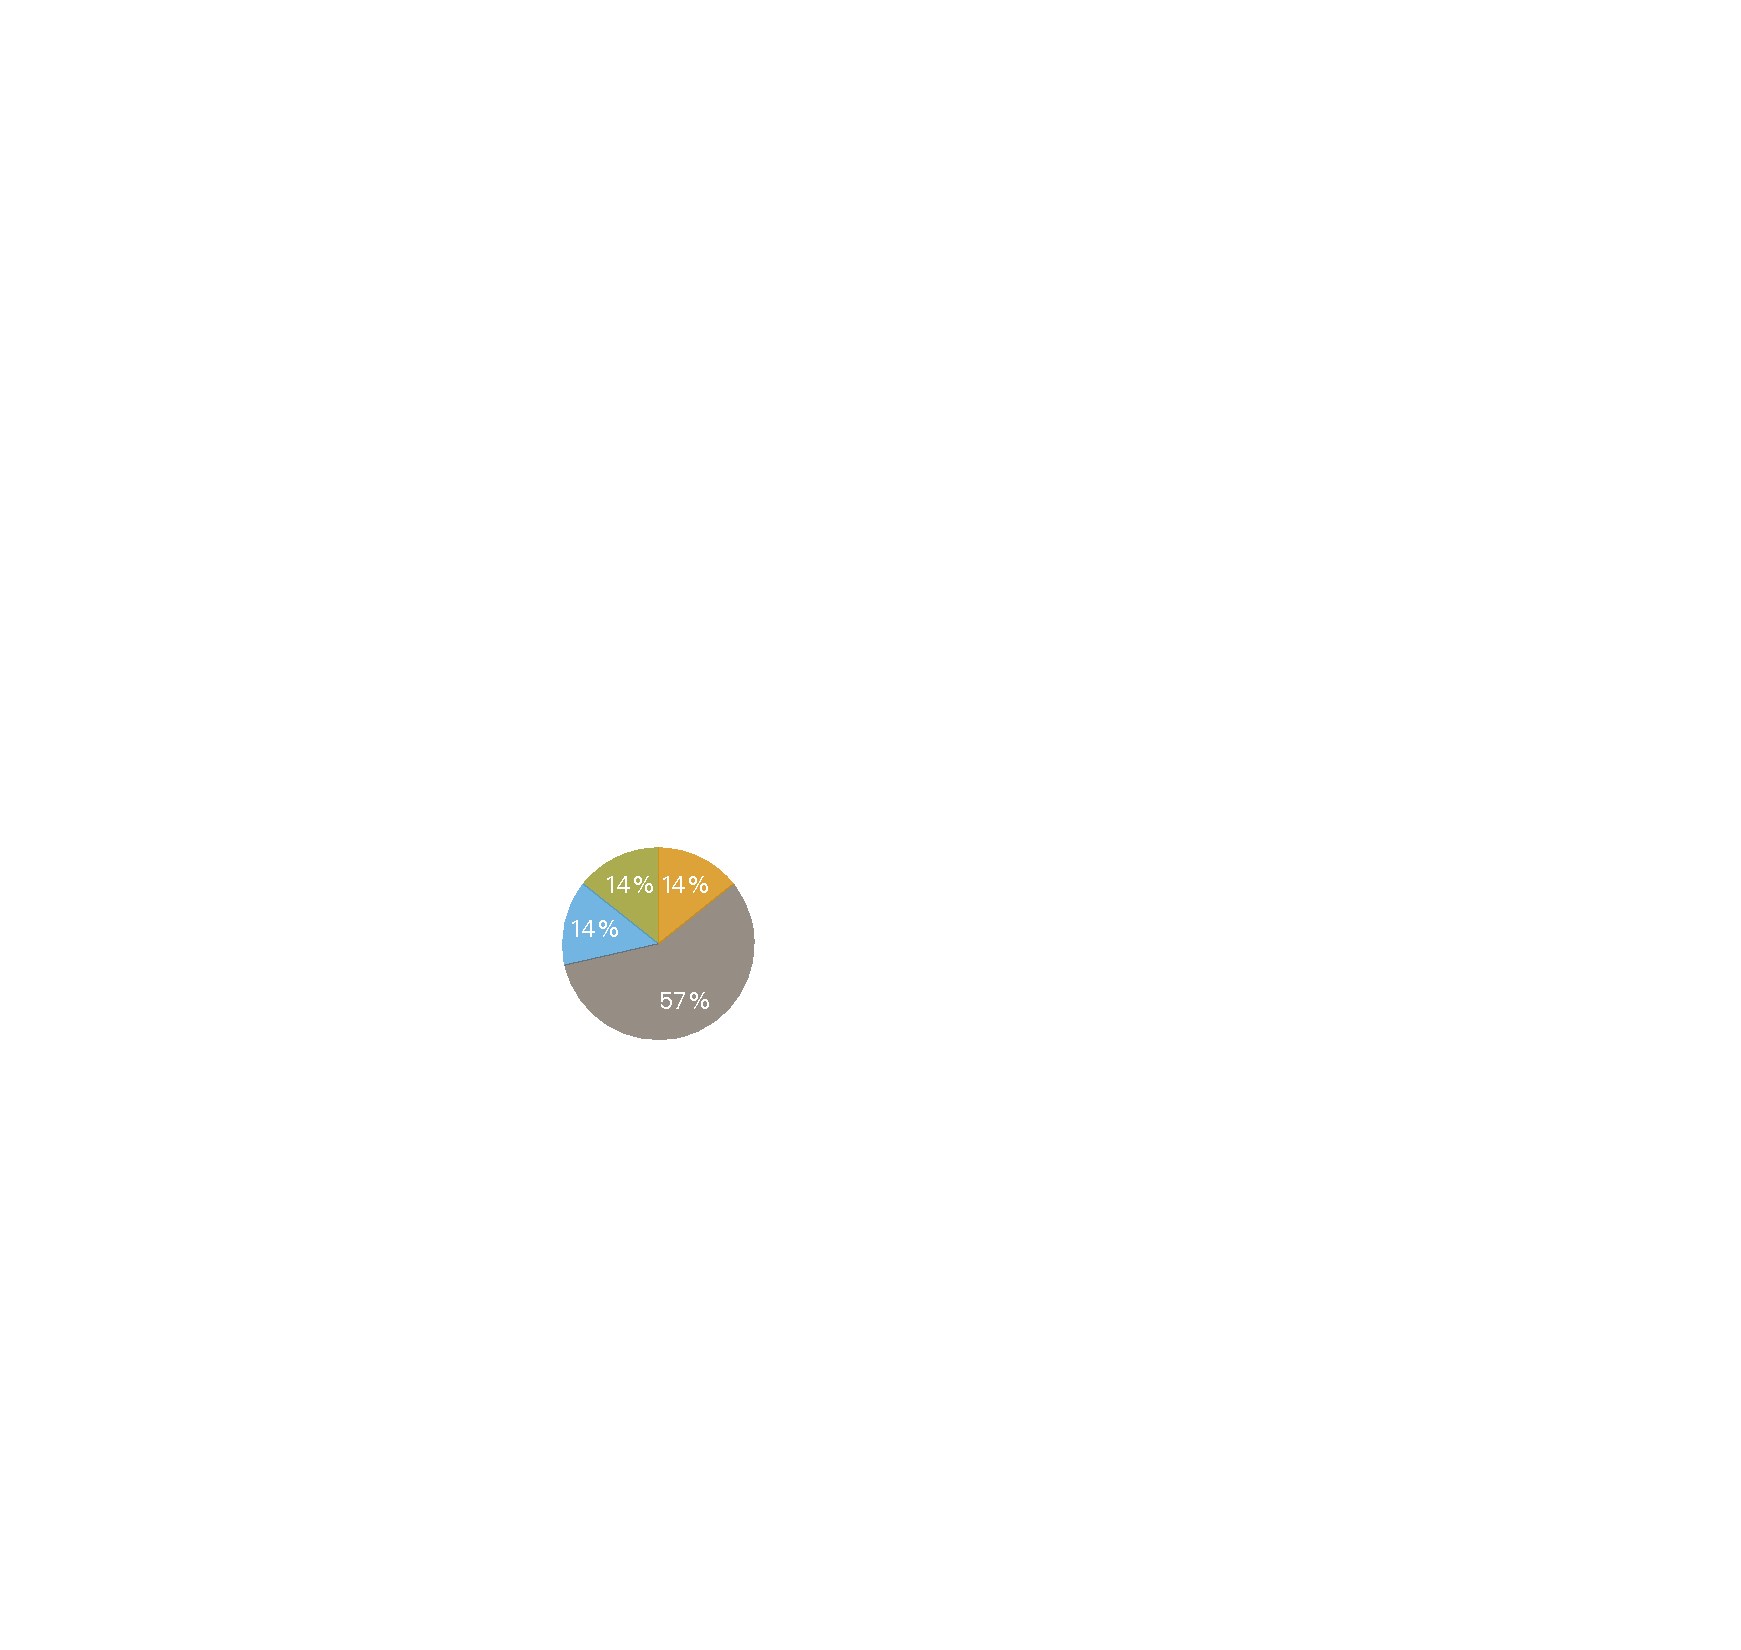
\includegraphics[scale=\graphicsscale]{resources/used-tools-charts-b}
        \caption{Präsentationsprogramme}
        \label{fig:used-tools-charts-b}
    \end{subfigure}
    \begin{subfigure}{\subfigurewidth}
        \centering
        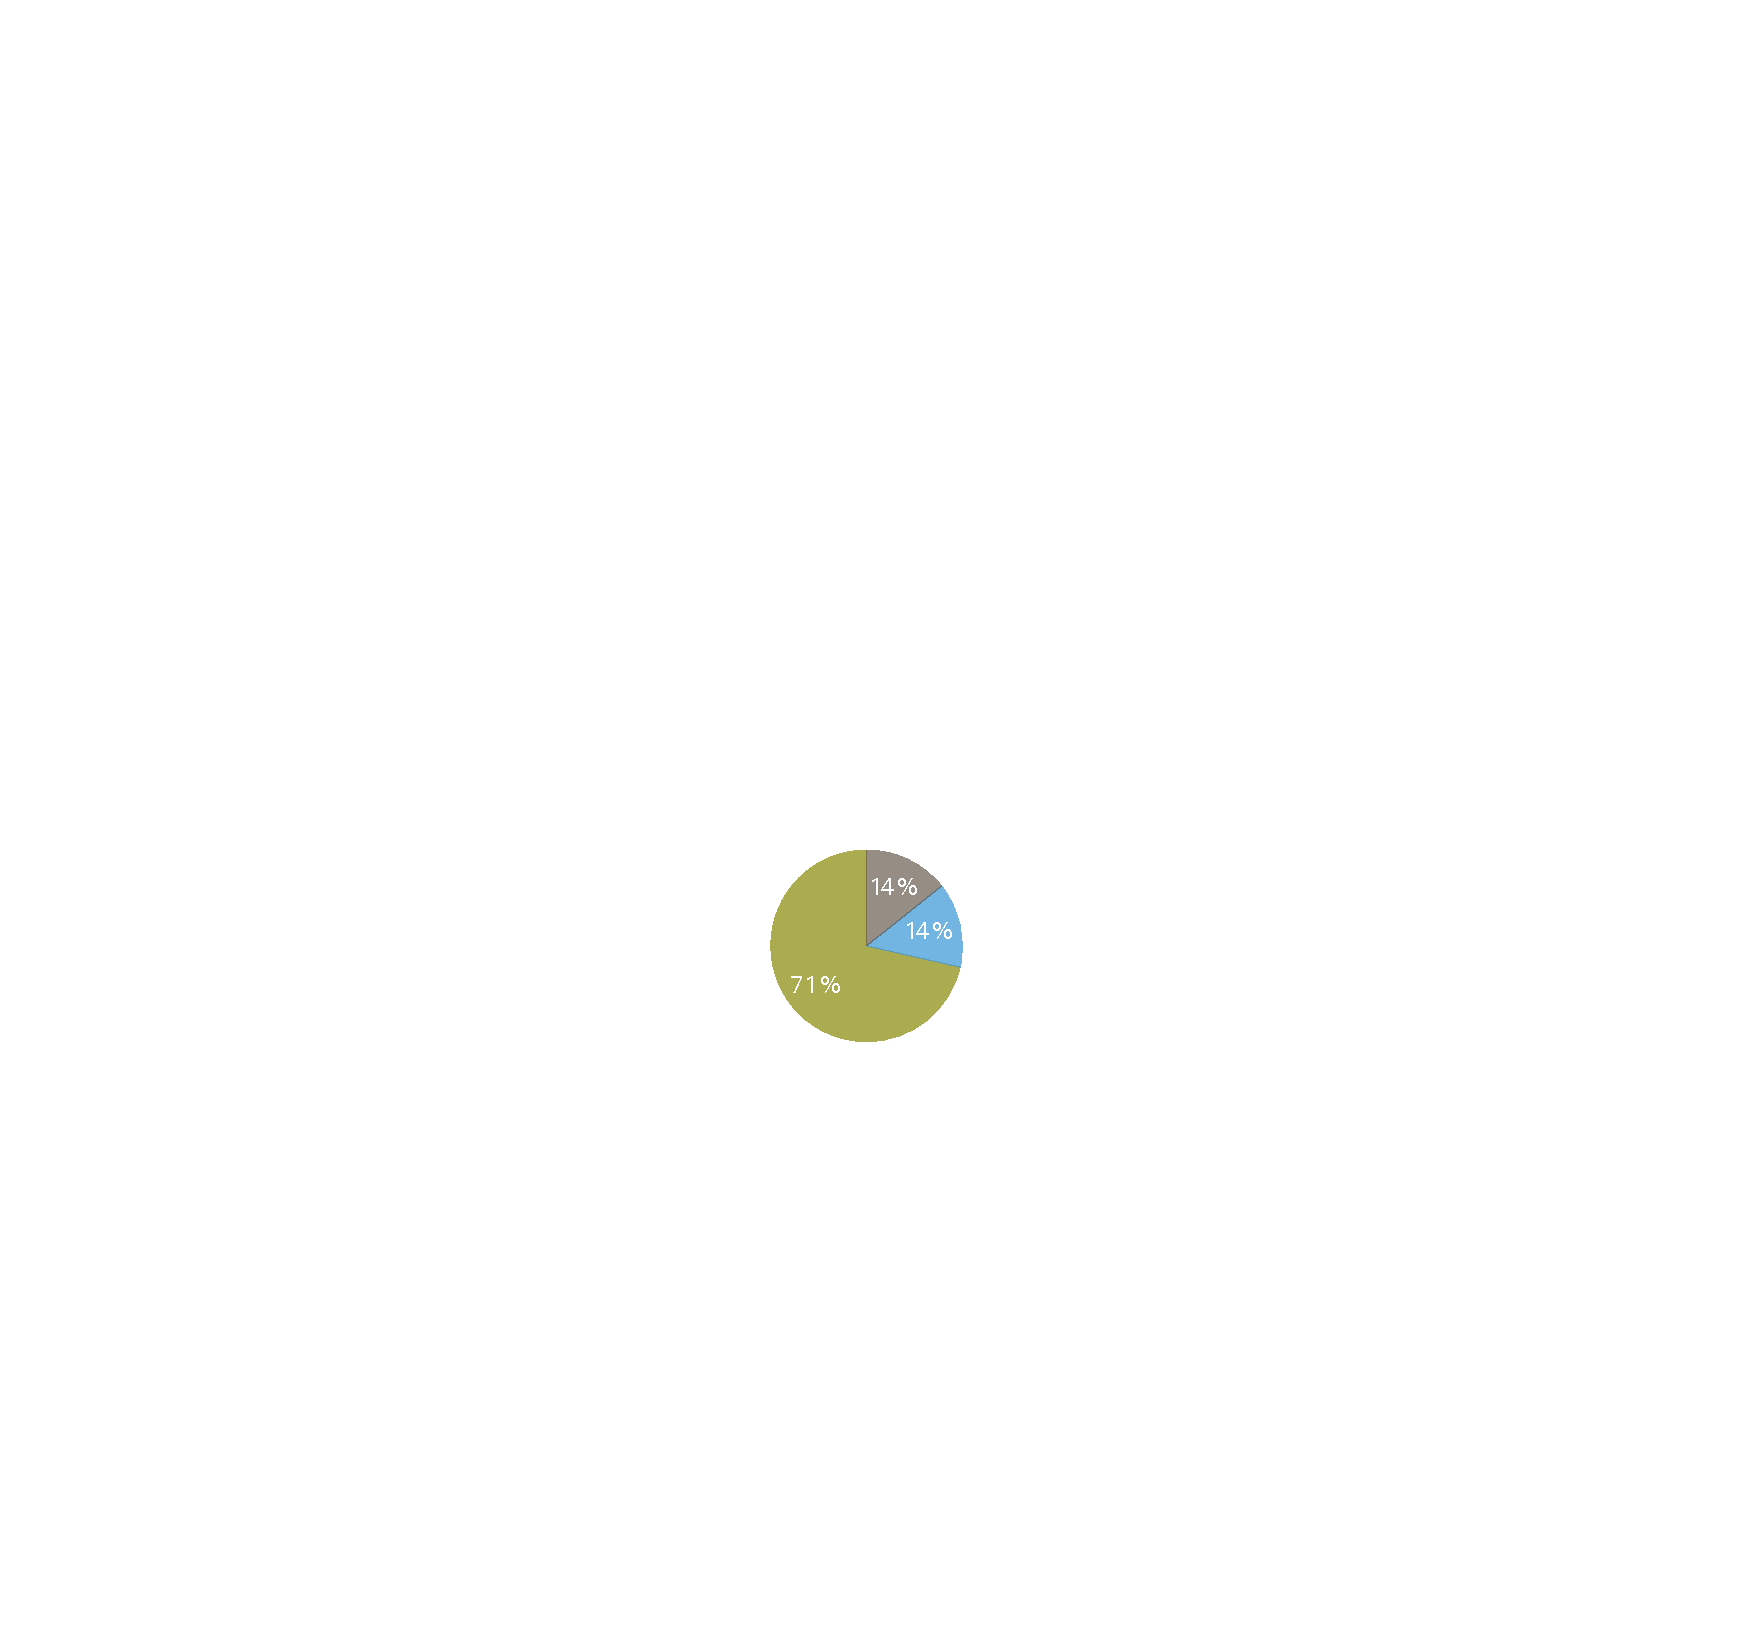
\includegraphics[scale=\graphicsscale]{resources/used-tools-charts-c}
        \caption{Online-Tools}
        \label{fig:used-tools-charts-c}
    \end{subfigure}
    \begin{subfigure}{\subfigurewidth}
        \centering
        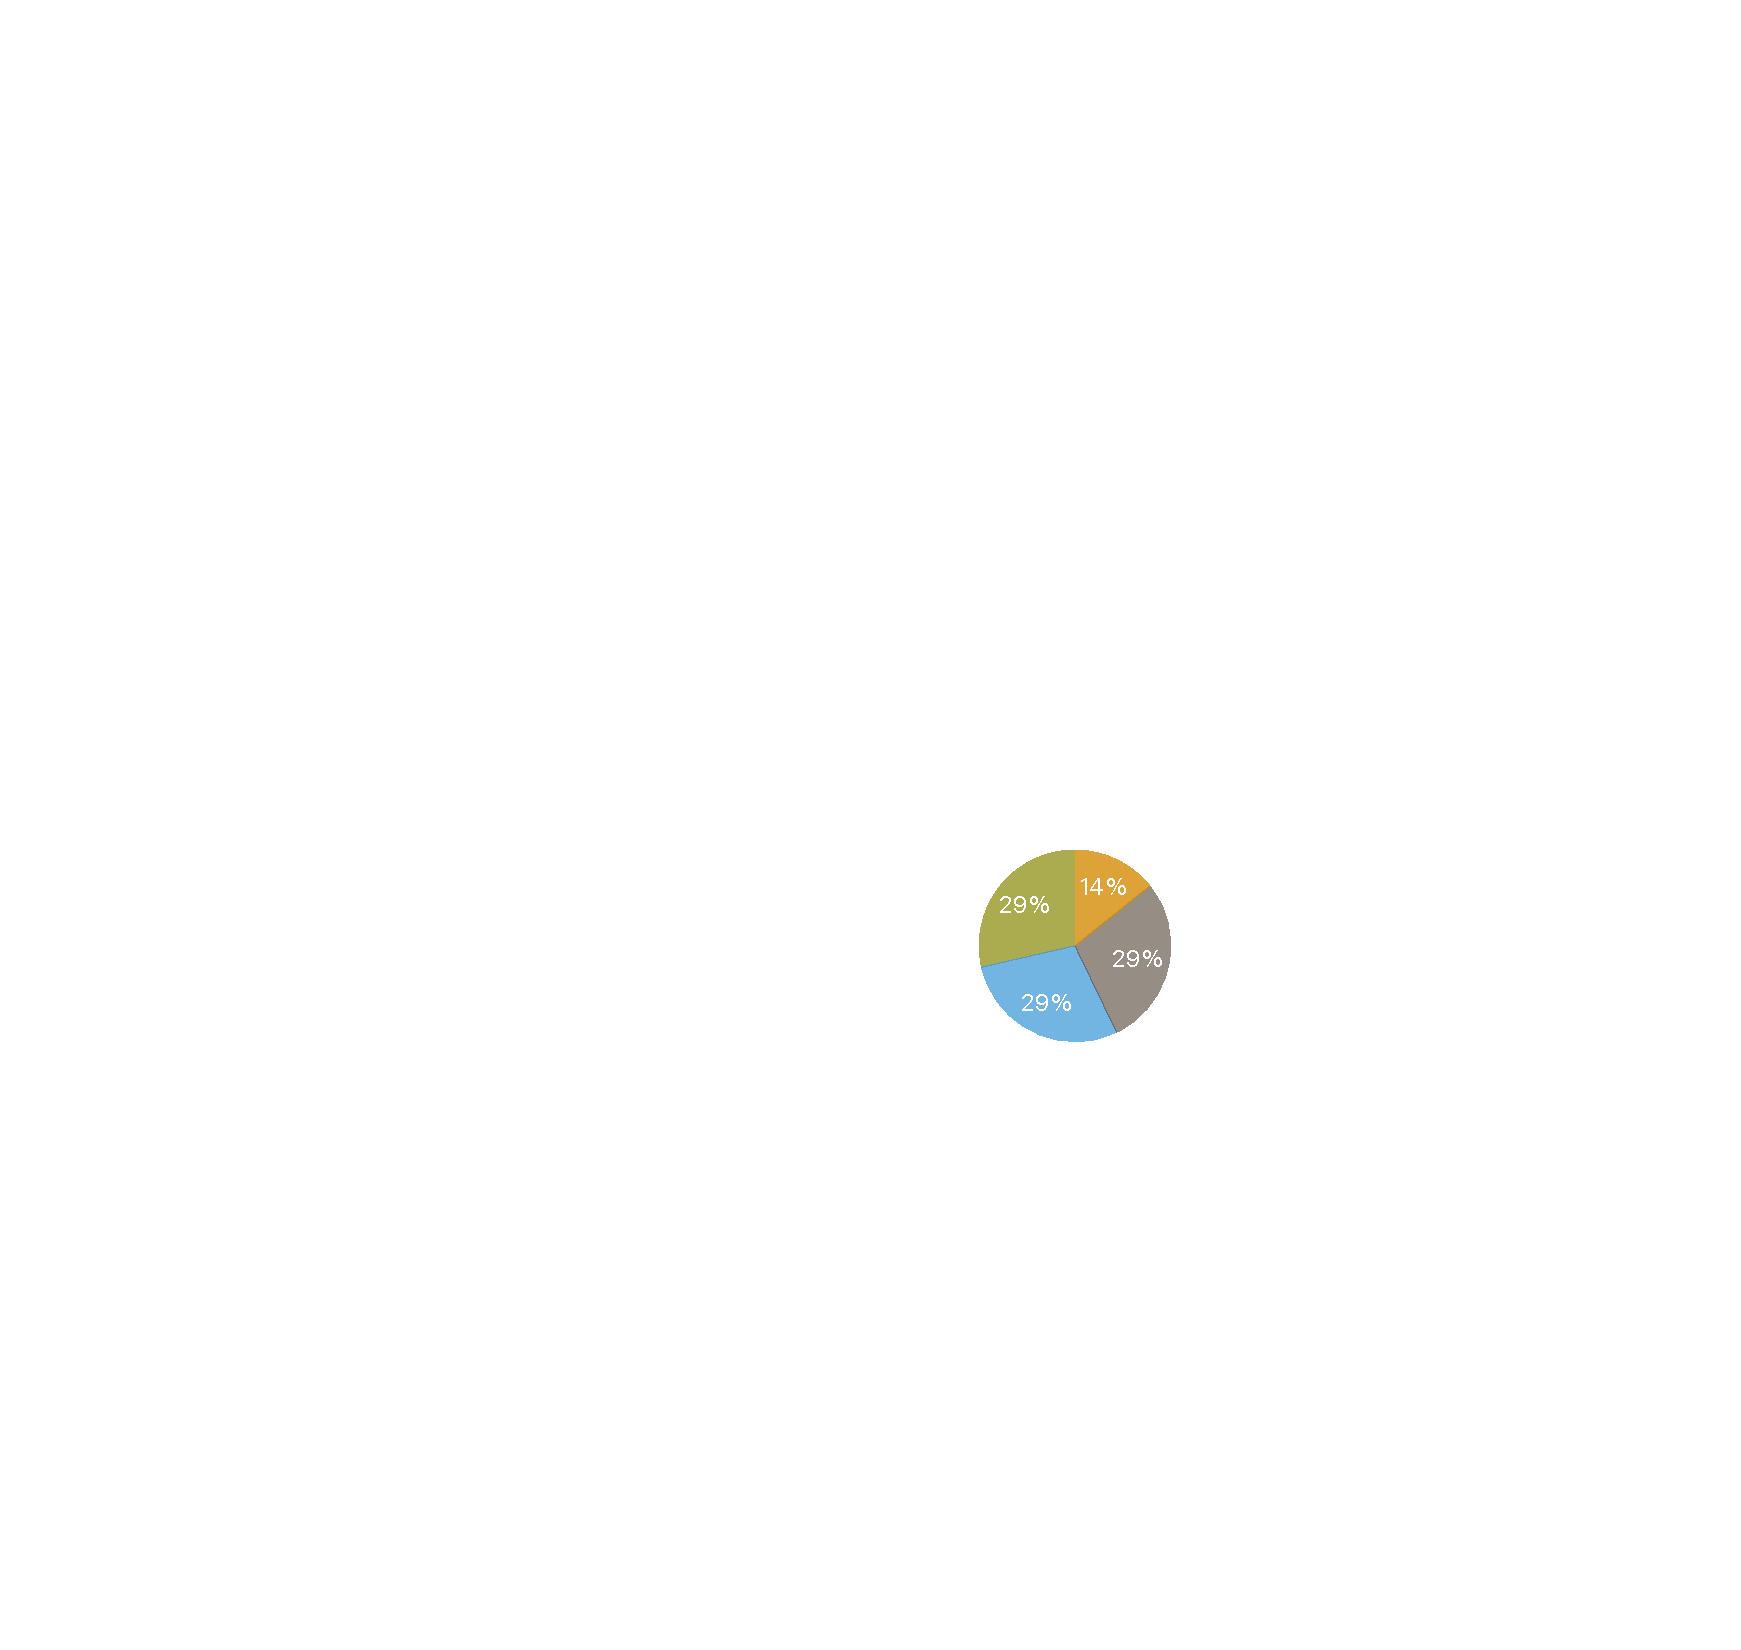
\includegraphics[scale=\graphicsscale]{resources/used-tools-charts-d}
        \caption{UML-Editoren}
        \label{fig:used-tools-charts-d}
    \end{subfigure}
    \begin{subfigure}{\subfigurewidth}
        \centering
        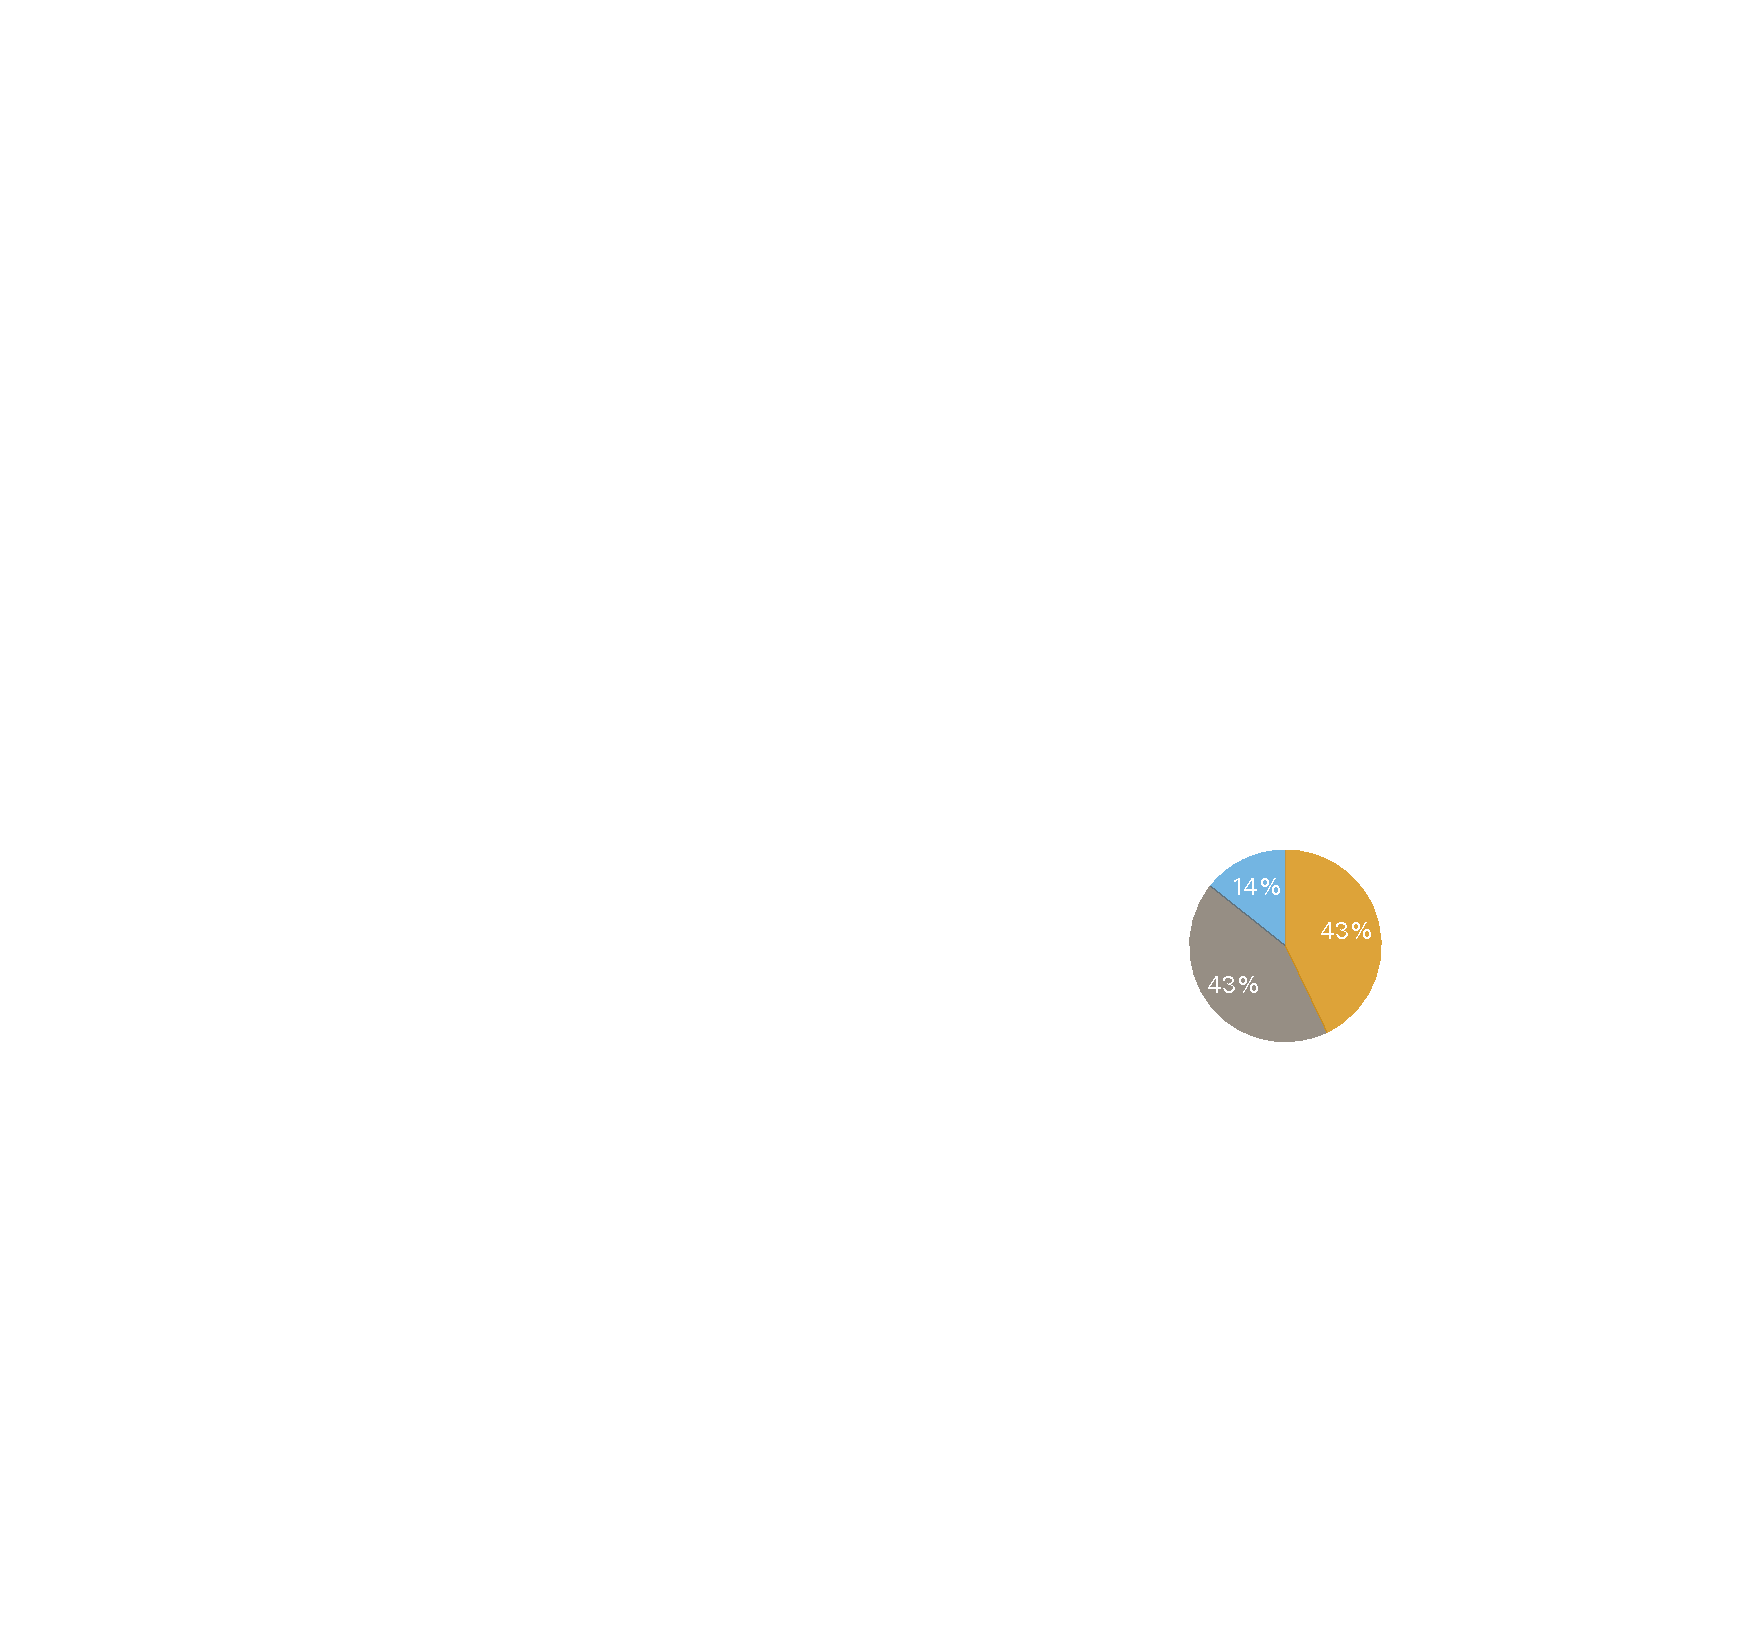
\includegraphics[scale=\graphicsscale]{resources/used-tools-charts-e}
        \caption{Stift und Papier}
        \label{fig:used-tools-charts-e}
    \end{subfigure}
    \begin{subfigure}{\subfigurewidth}
        \centering
        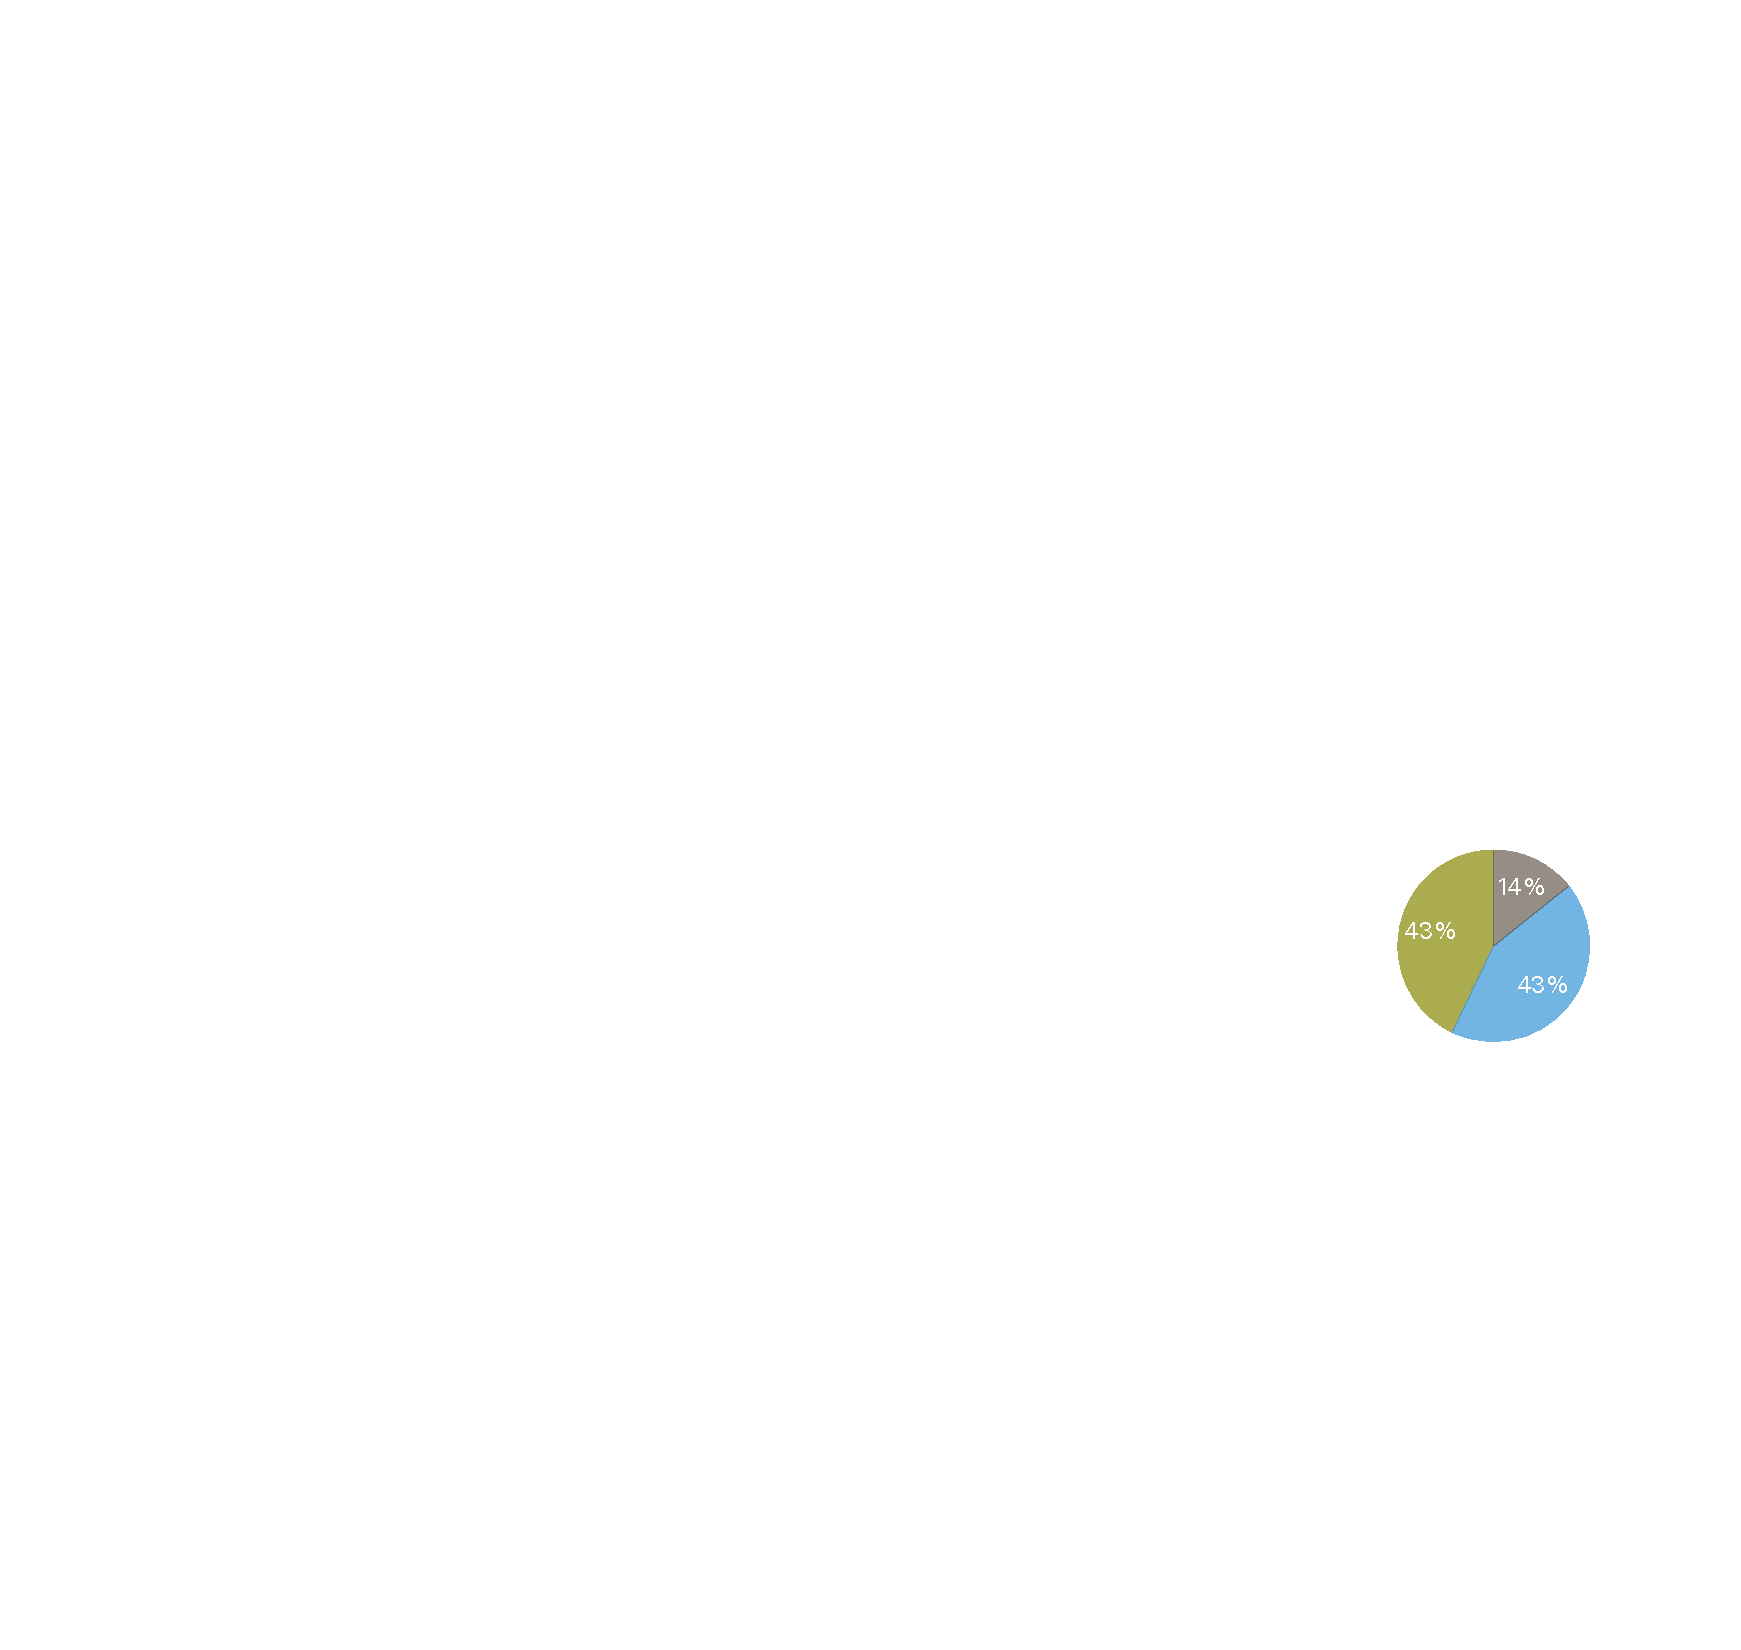
\includegraphics[scale=\graphicsscale]{resources/used-tools-charts-f}
        \caption{Whiteboard}
        \label{fig:used-tools-charts-f}
    \end{subfigure}
\end{minipage}
\caption{Auswertung der verwendeten Tools zum Erstellen von Diagrammen}
\label{fig:used-tools-charts}
\end{figure}

% andere Möglichkeit: keine Erklärung, aber Anlernen notwendig

% Beobachtungen
% Ergebnisse und Auswertung des Fragebogens
% Interpretation der Beobachtungen und Ergebnisse

% Fehlende Aktionen im Prototyp

\section{Zusammenfassung}
